%!TEX root = ../document.tex
\chapter{Anforderungsanalyse}
\label{ch:requirements}

Anforderungsanalyse wird von \cite[S. 598]{Balzert.2009} als \enquote{systematische Ermittlung, Beschreibung, Modellierung und Analyse von Anforderungen} definiert -- dieses Kapitel soll aufzeigen, welche Anforderungen an ein Suchsystem gestellt werden. Neben der Motivation für die Sammlung der Requirements wird primär das Vorgehen hierzu erläutert, beispielsweise welche verschiedenen Anforderungsquellen beachtet werden.

\section{Motivation}

\myMarginnote{Weshalb ist Requirements Engineering von Bedeutung für die Auswahl der Suchlösung?}
Zu Beginn der Suche nach Anforderungen steht die Frage, welchen Mehrwert \emph{Requirements Engineering} für das Projekt bedeutet.

\cite[S.7]{Pohl.2008} zählt Requirements Engineering zu den zwingenden Prämissen für erfolgreiche Softwareprojekte.

Eine Studie zum Thema \enquote{Erfolg und Scheitern im Projektmanagement} der GPM\footnote{GPM Deutsche Gesellschaft für Projektmanagement e. V.} untersuchte, welche Faktoren den größten Einfluss auf den Erfolg eines Projektes haben. Hierzu wurden 79 Unternehmen aus unterschiedlichen Branchen befragt. \enquote{Unklare Anforderungen und Ziele} wurden in den Studienergebnissen als zweithäufigste Ursache für gescheiterte Projekte genannt \cite[S. 3, 8]{GPMDeutscheGesellschaftfurProjektmanagemente.V..2008}.

Schlussendlich ist klar: Ohne zu wissen, was eine Search Engine für ReEvent leisten soll, ist es auch nicht möglich eine Evaluation durchzuführen oder eine Empfehlung abzugeben.

\section{Klassifizierung von Anforderungen}
\label{sec:require.classes}
Anforderungen werden gängigerweise in \emph{funktionale} und \emph{nicht funktionale}\footnote{\cite[S. 16]{Pohl.2008} nennt nicht funktionale Anforderungen auch Qualitätsanforderungen, beziehungsweise unterteilt nicht funktionale Anforderungen in funktionale und Qualitätsanforderungen} unterschieden. Funktional ist eine Anforderung dann, wenn sie sich auf eine Funktion oder ein Verhalten bezieht, welche das System leisten soll. Nicht"=Funktionale Anforderungen stellen Qualitätsmerkmale dar -- übliche Punkte sind hier Ausfallsicherheit oder Performanz. Zusätzlich können auch \emph{Randbedingungen} vorliegen, die zwar vom das System eingehalten werden müssen, aber keine Funktion oder Qualitätsfaktoren darstellen \cite[S. 8f]{Pohl.2015}. Beispiele hierfür sind die Kostenplanung oder gesetzliche Einschränkungen.

Eine weitere Klassifizierung, welche die Kunden- oder Benutzerzufriedenheit im Blick hat, stellt das Kano"=Modell dar. \emph{Basismerkmale} sind Funktionen, welche vom Produkt erwartet werden, etwa weil diese Funktion marktüblicher Standard sind. Systeme im Betrieb wie in Abschnitt \ref{sec:requirements_existing} können als Quelle für diese Anforderung dienen. Was der Kunde explizit fordert -- möglicherweise in der Form eines Lastenheftes -- wird unter \emph{Zusatzmerkmale} zusammengefasst. Systemeigenschaften, die über das hinausgehen, was der Kunde erwartet stellen \emph{Begeisterungsmerkmale} dar. Während Basismerkmale für das Produkt zwingend umgesetzt werden müssen, steigert die Umsetzung von Begeisterungsmerkmalen die Kundenzufriedenheit noch stärker als die der Zusatzmerkmale \cite[S. 534]{Pohl.2008}.

Die grundlegende Suchfunktion -- Abbildung einer Suchanfrage auf eine Treffermenge, die die Suchanfrage enthalten -- kann als Basismerkmal einer Suchmaschine aufgefasst werden. Unter Beachtung von Abschnitt \ref{sec:documents} und \ref{sec:requirements_insite} ist die Filterung von Veranstaltungen nach Datum ein Zusatzmerkmal. \emph{Natural Language Searching}\footnote{ein Teilbereich der Computerlinguistik} -- die semantische Analyse eines Suchbegriffes und dem Versuch die Intention des Benutzers herauszulesen -- könnte in diesem Zusammenhang als Begeisterungsmerkmal bezeichnet werden \cite[S. 6]{Aksyonoff.2011}. So könnten aus der Anfrage \enquote{Sportveranstaltung in der Saturn"=Arena} automatisch Filterkriterien für die Veranstaltungskategorie(Sport) und den Ort(Saturn"=Arena) gewonnen werden.

\section{Anforderungsquellen}

Um Anforderungen für ein spezifisches Projekt zu ermitteln, müssen verschiedene Aspekte des Projektumfeldes beachtet werden, welche das geplante System beeinflussen könnten.

\subsection{Identifikation der Stakeholder}

Einzelpersonen oder Gruppen, welche vom Projekt betroffen sind oder auf dieses Einfluss ausüben, werden \emph{Stakeholder} genannt \cite[S. 21]{Pohl.2015}.


\subsubsection{Veranstaltungsbesucher}

Veranstaltungsbesucher -- ob potentiell oder nicht -- suchen nach Veranstaltungen, für die sie ein Interesse hegen. Eine Recherche starten sie, weil sie eine bestimmte, kommende Veranstaltung besuchen möchten, Informationen für eine vergangene Veranstaltung einholen möchten -- beispielsweise Kontaktdaten der Organisatoren -- oder einfach ins Blaue hinein nach Events für die zugehörige Zielgruppe suchen.

Es wird angenommen, dass diese Gruppe verhältnismäßig den größten Anteil der Suchanfragen durchführt. In Abhängigkeit des Recherchebedürfnisses und des Interesses an Veranstaltungen steigt oder fällt dadurch auch die Menge der Suchanfragen -- somit auch die Auslastung des Suchservers.

\myMarginnote{\enquote{Welche Veranstaltungen finden in meiner Nähe statt?}}
Ein mögliches Feature könnte die Umkreissuche sein: Veranstaltungen wird in ReEvent ein Veranstaltungsort zugewiesen, der üblicherweise über GPS"=Koordinaten verfügen kann\footnote{Eine Ausnahme hiervon stellen beispielsweise sogenannte \emph{Webinare} dar. Das Kofferwort aus Web und Seminar beschreibt nach Duden ein \enquote{online stattfindendes Seminar}, der Veranstaltungsort wird durch eine URL definiert.}. Anhand des ermittelten, aktuellen Standortes des Benutzers oder durch einer vom Benutzer gewählten GPS"=Position und eines Maximalabstandes können Veranstaltungen gefiltert werden, die nicht in Reichweite des Benutzers liegen. Der Fachbegriff hierfür lautet \emph{geospatial search} \cite[S. 521]{Grainger.2014}.

Schließlich ist es grundlegendes Ziel jedes Veranstaltungsbesuchers, bei der Suche Veranstaltungen zu finden, die seinen Interessen -- und damit auch seiner Suchanfrage -- entsprechen. Außerdem liegt es nahe, den Präferenzen des Nutzers entsprechend einzelne Veranstaltungen vorzuschlagen, die der Benutzer andernfalls verpassen könnte. Um die User Experience nicht zu beeinträchtigen, sollten Anfragen an die Suchmaschine nicht um ein Vielfaches länger dauern als andere Seitenaufrufe auf diesem Server.

\subsubsection{Veranstalter}

Auch Organisatoren von Veranstaltungen können ReEvent durchsuchen. In erster Linie werden die eigenen Veranstaltungen Ziel der Suche sein, da der öffentliche Eintrag in ReEvent eine Informationsquelle für Besucher darstellt. Falls Korrekturen an diesem Eintrag notwendig werden und der Veranstalter überprüfen möchte, ob diese bereits durchgeführt wurden, könnte er diese Veranstaltung über die Suche aufrufen.

Ebenfalls im Blickpunkt eines Veranstalters sind \emph{ähnliche} Veranstaltungen zu den Eigenen. Um das Publikum für die Veranstaltung nicht aufzuteilen, könnte es im Sinne des Veranstalters sein, eigene Veranstaltungstermine nicht gleichzeitig zu ähnlichen Konkurrenzveranstaltungen zu legen. Führen beispielsweise zwei Zirkusunternehmen gleichzeitig Vorstellungen am selben Ort auf, so würde sich der durchschnittliche Besucher für eines der beiden entscheiden.

Einen weiteren Berührpunkt mit dem Suchsystem haben Veranstalter in Bezug auf die Anzahl der Veranstaltungen. Je nachdem wie viele Veranstaltungen durchgeführt werden, muss das Suchsystem auch eine andere Menge an Veranstaltungen handhaben.

\subsubsection{Editoren}

Ähnlich wie auch Veranstalter könnten auch Backend"=Nutzer von ReEvent Events im Fokus haben, welche sie persönlich erstellt oder editiert haben. Insbesondere um die Auswirkungen einer Änderung im Frontend zu überprüfen, wäre eine Filterung nach \enquote{zuletzt bearbeitet von} sinnvoll.\footnote{alternativ sollte im Backend für jede Veranstaltung eine Verlinkung für die entsprechende Seite im Frontend enthalten sein}

Sowohl Änderungen als auch Neueintragungen sollten daher sofort oder sobald wie möglich von der Suche erfasst werden.


\subsection{Bestimmung des Systemkontextes}

\cite[S. 85-87]{Rupp.2014} teilt die Umgebung eines Projektes in drei Bereiche ein: den \emph{Scope} des zu erstellenden Systems, den \emph{Systemkontext} und den \emph{irrelevanten} Teil der Umgebung. Der Systemkontext entspricht denjenigen Teil des Umfeldes, welcher für die Erstellung und Interpretation des Projektes von Bedeutung ist \cite[S. 55]{Pohl.2008}. Währenddessen wird die irrelevante Umgebung -- wie der Name bereits vermuten lässt -- im weiteren Verlauf des Requirements Engineering ausgeblendet \cite[S. 462]{Balzert.2009}.

\begin{figure}[ht!]
\begin{margincap}
\centering
\begin{tikzpicture}
	\fill[fill=halfgray] (0,0) ellipse (2.5cm and 2cm);
	\fill[fill=titlepagecolor] (-0.7,0) circle (1cm) node[color=white] {\sffamily Scope};
	\node[color=white,align=center] at (1.4,0) {\sffamily System-\\\sffamily kontext};
	\node[align=center] at (4,1) {\sffamily irrelevante\\\sffamily Umgebung};
\end{tikzpicture}
\caption[Scope, Systemkontext und irrelevante Umgebung]{Scope, Systemkontext und irrelevante Umgebung nach \cite[S. 86]{Rupp.2014}}
\label{img:systemcontext}
\end{margincap}
\end{figure}

Der Systemkontext soll gemäß \cite[S. 461]{Balzert.2009} festgelegt werden, da die in ihm enthaltenen Objekte Einfluss auf Anforderungen an das eigentliche System nehmen können.

\subsubsection{ReEvent}
\label{sec:requirements_reevent}
Mit ReEvent als Quelle für die zu durchsuchenden Daten steht bereits ein Teil des Systemkontextes fest. Entsprechend können die Inhalte des Kapitels \ref{ch:reevent} wieder aufgegriffen und hinsichtlich möglichen Anforderungen untersucht werden. Die eingetragenen Veranstaltungen enthalten primär Textfelder, wie den Namen der Veranstaltung sowie Beschreibungstexte. Hierbei ist es möglich, dass insbesondere Beschreibungsfelder eine Auszeichnungssprache wie HTML oder Markdown enthalten. Die primäre Aufgabe des Suchsystems soll eine Volltextsuche über diese Daten sein. \myMarginnote{Durchsuchung von Anhängen im PDF"= oder Word"=Format} Des Weiteren können zusätzliche Dateien angefügt werden.\footnote{vergleiche Abschnitt \ref{sec:reevent_about}} Diese können unterteilt werden in textbasierte Formate und solche ohne Textinformationen. Zur ersten Kategorie kann man entsprechende PDF- oder Microsoft Word"=Dokumente zählen, aber auch andere Formate wie HTML oder XML sind prinzipiell maschinenlesbar. Möglicherweise müssen diese Dateien jedoch aufbereitet werden. Ebenfalls möglich ist die Abspeicherung weiterer Dateitypen, die nicht in erster Linie textbasiert sind. Hier kommen in erster Linie Medien wie Bilder, Sound oder Videos in Betracht. Diese verfügen aber meist über Metadaten -- so können MP3"=Dateien über sogenannte \emph{ID3"=Tags} mit Informationen zu Künstler, Album und Liedtitel angereichert werden.

Insbesondere bei Bilddateien kann man noch einen Schritt weitergehen: durch Verfahren der \emph{Optical Character Recognition} können aus diesen wiederum Textinformationen gewonnen werden. Enthält das Bild beispielsweise ein Namensschild oder stellt es eine Aufnahme einer Speisekarte dar, so besteht mittels OCR die Möglichkeit, dass diese Informationen aus der Grafik ausgelesen und anschließend für die Suche bereitgestellt werden können.

Die Oberfläche von ReEvent -- sowohl im Backend als auch im Frontend -- kann lokalisiert werden. Das Suchformular sowie die Auflistung der Suchergebnisse sollten ebenfalls entsprechend angepasst werden können.

\myMarginnote{Mehrsprachige Inhalte}
Ebenfalls ein Kriterium stellen die mehrsprachig eingetragen Texte dar: Wie in Abschnitt \ref{sec:ReEvent:MultiLanguage} gezeigt, können Veranstaltungen übersetzt werden. Das Suchsystem muss somit in der Lage sein, Varianten ein und derselben Veranstaltung, aber in einer anderen Sprache zu indizieren und zu durchsuchen. In erster Linie werden Veranstaltungen der Stadt Ingolstadt in deutscher Sprache abgefasst werden, mit einem gewissen Anteil ins Englische übertragener Events ist zu rechnen. Da die Stadt Ingolstadt Städtepartnerschaften unter anderem zu Moskau(Russland), Legmoin(Burkina Faso) und Foshan(China) pflegt, kommen auch die zugehörigen Landessprachen in Betracht \cite{StadtIngolstadt.2014}. Insbesondere das Chinesische als \emph{CJK Sprache} könnte eine potentielle Schwierigkeit für ein Suchsystem darstellen \cite[S. 95f]{Buttcher.2010}.

\myMarginnote{Mehrere Varianten durch Workspaces und zeitpunktabhängige Daten}
Auch das Konzept der Workspaces stellt eine Herausforderung für ein Suchsystem dar. Da theoretisch für jeden Editor eine Instanz eines jeden Objektes existieren kann, beläuft sich die Gesamtsumme auf $n+1$ Varianten bei $n$ Editoren, auch der globale, beziehungsweise öffentliche Workspace muss dazu gezählt werden. Für diese Situation existieren zwei unterschiedliche Ansätze.

\begin{itemize}
	\item Suche für \emph{alle} Workspaces
	\item Reduktion auf den globalen Workspace
\end{itemize}

Wenn alle Workspaces durchsucht werden sollen, kann der Aufwand hierfür linear mit der Anzahl der Editoren ansteigen. Alternativ kann man den Scope der Suche auch einschränken: so können lediglich veröffentlichte Objekte durchsucht werden -- was aber den Vorteil hat, dass sich der Aufwand auf nur eine Variante dieses Objektes reduziert. Diese Entscheidung hat lediglich Auswirkungen auf das Backend, das Frontend hat schließlich nur Zugriff auf den öffentlichen Workspace. Im Backend könnten für die erste Variante sogar zwei Suchen angeboten werden: Eine für den privaten Workspace des angemeldeten Benutzers, sowie für den öffentlichen Workspace. Bei der der zweiten Möglichkeit sind dem Editor die eigenen Änderungen über die Suche nicht sichtbar. Es stellt sich somit die Frage, ob der Mehrwert für den einzelnen Editor den zusätzlichen Aufwand rechtfertigt.

Schlussendlich sollen auch die historischen Schritte aus Abschnitt \ref{sec:history.steps} für die Suche verfügbar sein. Hier liegt die grundlegende Problematik darin, dass jeder historischer Schritt eine kleine Abwandlung des Vorgängers darstellt. Würde man in der Suche jeden historischen Schritt getrennt voneinander betrachten, könnte folgendes Szenario auftreten.\footnote{in Anlehnung an \url{http://www.augsburger-allgemeine.de/neuburg/So-haelt-Ingolstadt-dagegen-id33881902.html}}

\begin{figure}[ht!]
\begin{margincap}
	\centering
	\begin{tikzpicture}
	\node[draw, align=left] (first) at (0,0) {Veranstaltung: Landesaustellung 2016 \\ Ort: Ingolstadt \\ Datum: 20.04.2016};
	\node[draw, align=left] (second) at (0,-2.5) {Veranstaltung: Landesaustellung 2016 \\ Ort: \colorbox{MarkerYellow}{Aldersberg} \\ Datum: 20.04.2016};
	\node[draw, align=left] (third) at (0,-5) {Veranstaltung: Landesaustellung 2016 \\ Ort: Aldersberg \\ Datum: \colorbox{MarkerYellow}{29}.04.2016};

	\node [left=of first] {Version 1};
	\node [left=of second] {Version 2};
	\node [left=of third] {Version 3};

	\node [font=\Large] at ($(first.south)+(0,-0.5)$){$\Downarrow$};
	\node [font=\Large] at ($(second.south)+(0,-0.5)$){$\Downarrow$};

	\end{tikzpicture}
	\caption[Historische Schritte am Beispiel einer Veranstaltung]{Historische Schritte am Beispiel einer Veranstaltung. Die jeweiligen Änderungen wurden gelb hinterlegt. Das Beispiel basiert lose auf der Vergabe der Landesausstellung 2016 mit dem Thema \enquote{Bier in Bayern}.}
	\label{fig:historic_steps_search_problem}
\end{margincap}
\end{figure}

Die Landesausstellung 2016 stellt eine -- mehr oder weniger -- einzigartige Veranstaltung dar, zumindest alle drei historische Schritte aus Abbildung \ref{fig:historic_steps_search_problem} beziehen sich im Grunde auf ein und dieselbe Veranstaltung. Würde man nun bei einer Suche nach \enquote{Landesaustellung 2016} diese historischen Schritte als eigenständige Objekte handhaben, so könnte die Ergebnisliste exakt diese drei Objekte als Treffer enthalten -- obwohl sie dieselbe Veranstaltung darstellen. Auch kann man die Suche nicht auf die aktuellste Version beschränken: Würde ein Benutzer, der noch nichts vom neuen Veranstaltungsort erfahren hat nach einer Landesausstellung in Ingolstadt suchen, würde er keinen Treffer erzielen. Somit wäre der Vorteil der historischen Schritte -- Nachvollziehbarkeit von realen Änderungen -- hinfällig.

ReEvent selbst basiert auf \emph{Neos CMS} und \emph{Flow}. Zur primären Datenhaltung wird das RDBMS \emph{MySQL} genutzt.\footnote{Das Datenbanksystem ist nicht zwingend gesetzt, vergleiche Abschnitt \ref{sec:reevent.database}} Das Suchsystem muss die Daten aus diesem Kontext erhalten, möglicherweise muss hierfür ein entsprechendes Importskript für die Kopplung der Systeme entwickelt werden.

Sowohl ReEvent als auch die zugehörige Datenbank werden auf virtualisierten Maschinen im \emph{Rechenzentrum} der Stadt Ingolstadt gehostet. Unter anderem werden hier die Betriebssysteme Windows Server 2008 und Debian verwendet. Sollte die Suchlösung auf einer eigenen Maschine innerhalb des Rechenzentrums installiert werden, müssen eventuell vorhandene Richtlinien des Rechenzentrums beachtet werden. Auch notwendige Netzwerkfreigaben\footnote{beispielsweise Portfreigaben} sind in Abstimmung mit dem Rechenzentrum einzurichten.

Da eine Search Engine möglicherweise auch für andere Seiten und Applikationen der Stadt nutzbar ist, könnten hierdurch Synergieeffekte entstehen. Ein Beispiel hierfür stellt die Hauptseite der Stadt Ingolstadt\footnote{siehe \url{http://www2.ingolstadt.de/}} dar, welche auf dem CMS IKISS der Firma Advantic basiert \cite{AdvanticSystemhausGmbH.2015}.\footnote{IKISS bietet bereits eine Volltextsuche, möglicherweise basierend auf Apache Solr}

\subsection{Bestehende Systeme}
\label{sec:requirements_existing}

Auch Vorgängersysteme oder Produkte der Konkurrenz können Quellen für Anforderungen darstellen \cite[S. 21]{Pohl.2015}. Benutzer sind an Funktionen dieser Software gewöhnt, sie erwarten somit ähnliche Funktionen und Funktionsweisen gegenüber dem neuen System. Zudem erleichtert es den Einstieg in die Arbeit mit dem neuen Produkt, wenn es sich ähnlich verhält wie vergleichbare Systeme.

\subsubsection{INsite}
\label{sec:requirements_insite}

Eine bedeutende Rolle für mögliche Anforderungen an das Suchsystem spielt auch das Altsystem INsite. Hierzu besteht die Möglichkeit, vorliegende Webserverlogs auszuwerten. Suchanfragen über das Frontend von INsite werden hierbei wie folgt geloggt:

\begin{listing}
\begin{minted}[breaklines]{text}
0.0.0.0 - [13/Nov/2015:00:13:55 +0100] GET /relaunch/veranstaltungen.cfm?regionString=&[...]&searchPhrase=&submit=Senden HTTP/1.0 200 249401
\end{minted}
\end{listing}

Alle Filter -- wie Beispielsweise \texttt{regionString} -- werden als GET"=Parameter an die URL angehängt. Im obigen beispielhaften Logeintrag wurden weitere Filter, welche üblicherweise mit übertragen werden durch das Auslassungszeichen [...] ersetzt. Die anfragende IP"=Adresse wird aus datenschutzrechtlichen Gründen nicht abgespeichert und durch einen Platzhalter 0.0.0.0 ersetzt. Ebenfalls protokolliert wird der Zeitstempel der Abfrage. Schließlich beinhaltet der Logeintrag auch den Parameter \texttt{searchPhrase}, welcher bei einer Suchanfrage den gesuchten Begriff enthält.

Hierzu wurden die Logdateien aus dem Zeitraum vom 06.03.2015 bis zum 15.11.2015 ausgewertet. Die Logeintrage, welche einen Suchbegriff enthalten, wurden durch einen regulären Ausdruck herausgefiltert.

\begin{equation*}
\underbrace{
	\text{
		\texttt{\textbackslash/relaunch\textbackslash/veranstaltungen\textbackslash.cfm}
	}
}_{\text{URL}}
\text{\texttt{.*?}}
\underbrace{
	\text{
		\texttt{searchPhrase=[\textasciicircum\&]}
	}
}_{\text{Suchbegriff}}
\end{equation*}

Der Regex"=Ausdruck schränkt die Ergebnismenge zuerst auf alle Einträge ein, welche die richtige URL enthalten. Anschließend wird überprüft, ob der Parameter \texttt{searchPhrase} enthalten ist und dieser einen Wert mit Länge ungleich Null hat. Dies geschieht durch Überprüfung des auf das Gleichheitszeichen folgende Zeichens: nur wenn dieses kein \& ist, wurde ein Suchbegriff übergeben. Das erste auf das Gleichheitszeichen folgende Et"=Zeichen ist stets der Trenner zum nächsten GET"=Parameter in der URL. Es kann somit niemals Teil eines Suchbegriffes sein, denn wenn Suchanfragen\footnote{oder auch sonstige GET"=Parameter} ein \& enthalten, so wird dieses in der URL zu \texttt{\%26} kodiert.


\begin{figure}[ht!]
\begin{margincap}
\centering
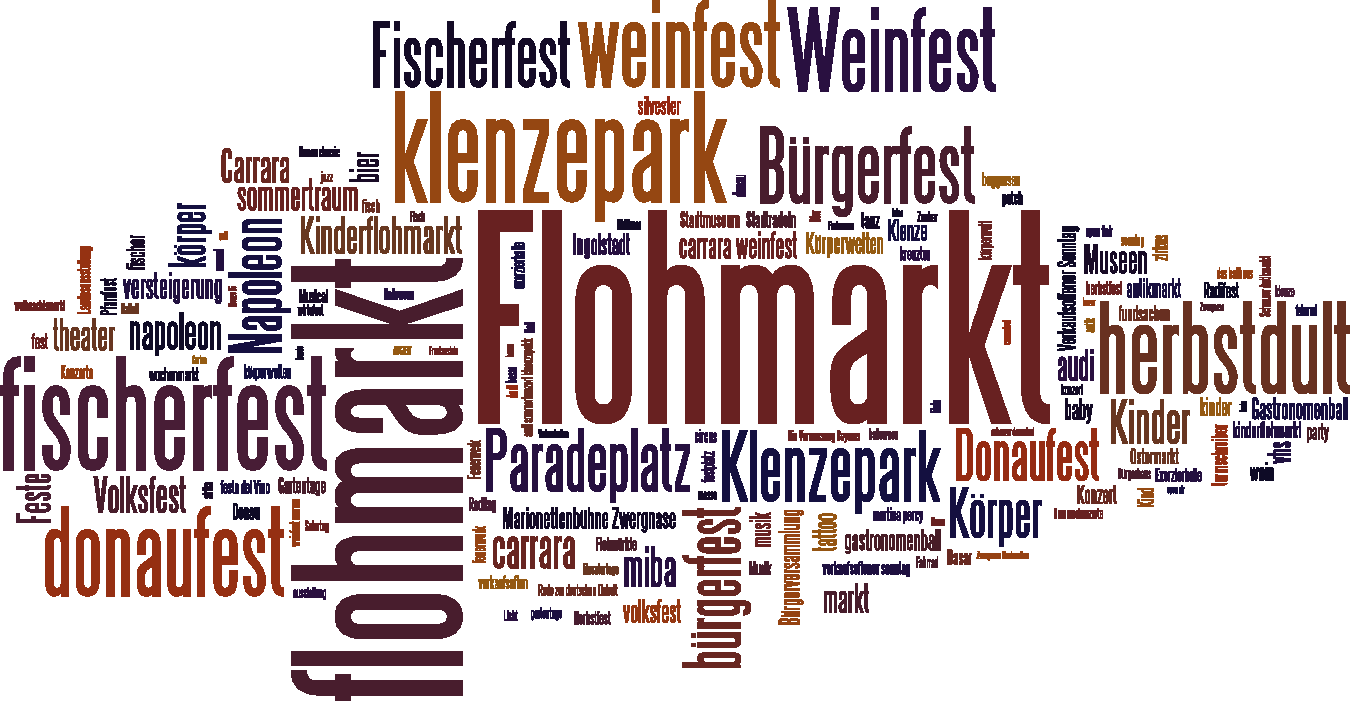
\includegraphics[width=\textwidth]{searchwords_cloud.pdf}
\caption[Häufige Suchbegriffe]{Eine Auflistung der Suchbegriffe im Frontend von INsite. Die Schriftgröße korreliert hierbei mit der Häufigkeit des Suchbegriffes. Angezeigt werden nur Begriffe, welche mindestends dreimal angefragt wurden. Die Grafik wurde mit Hilfe des Java"=Applets unter \url{http://wordle.net} erstellt.}
\label{img:searchword_cloud}
\end{margincap}
\end{figure}



Insgesamt wurden im genannten Zeitraum \numprint{2632} Suchanfragen getätigt. Verteilt über \numprint{254} Tage ergeben sich somit
\begin{equation}
\frac{Suchanfragen}{Zeitraum} = \frac{2632}{254 d} \approx 10,36 \frac{1}{d}
\end{equation}
Suchanfragen pro Tag.

Die Abbildung \ref{img:searchword_cloud} zeigt die aus den Logs extrahierten Suchbegriffe. Die Schriftgröße stellt dabei ein Maß für die Häufigkeit einer Anfrage dar. Fehler bei der Groß- und Kleinschreibung oder weitergehende Rechtschreibfehler wurden nicht korrigiert. Dies wird an den prominentesten Begriffen \emph{Flohmarkt} und \emph{flohmarkt} sichtbar, welche jeweils 79 beziehungsweise 64 Suchanfragen repräsentieren.

\myMarginnote{Werden Operatoren genutzt?}
Lediglich 15 Suchanfragen enthalten Sonderzeichen wie +, \#, \% oder *, welche in anderen Suchsystemen erweiterte Funktionen bereitstellen können -- \% und * werden beispielsweise als Wildcard"=Operatoren verwendet \cite[S. 111]{Wieken.2009}. Gängige boolesche Operatoren wie \texttt{AND} oder \texttt{OR} sind nicht enthalten. Da die INsite"=Suche auf dem SQL"=Operator \mintinline{sql}{LIKE} basiert, ist hiervon lediglich das \%-Zeichen von Relevanz. Die Verwendung von derartigen Sonderzeichen lässt auf ein entsprechendes Vorwissen um Volltextsuche schließen. Da der Anteil dieser Anfragen jedoch verschwindend gering ist, kann auch von einem geringen Prozentsatz vergleichsweise fortgeschrittener Benutzer ausgegangen werden.

Eine Untersuchung mit der Rechtschreibüberprüfung \emph{hunspell} ergab einen Anteil von 69\,\% fehlerhaften Suchanfragen. Hierbei ist jedoch zu beachten, dass hiervon Groß- und Kleinschreibfehler sowie von \emph{hunspell} nicht erkannte Eigennamen einen großen Teil beitragen. Dennoch sind auch zahlreiche Rechtschreibfehler enthalten. Dies lässt die Schlussfolgerung zu, dass eine automatische Korrektur von Rechtschreibfehlern einen Mehrwert für die Suche darstellt.


Weitergehende Untersuchung der Logeinträge zeigt, dass innerhalb eines Zeitintervalls von fünf Sekunden maximal vier Suchanfragen getätigt wurden.\footnote{Diese Untersuchung wurde über ein Java"=Programm durchgeführt, welches für jeden Zeitstempel aus den Logdateien überprüft, von wie vielen weiteren Zeitstempeln er innerhalb eines Zeitraums von \numprint{5000} Millisekunden umgeben ist.} Für das Intervall wurden fünf Sekunden gewählt, da Anfragen an den Server -- beziehungsweise die Suchmaschine -- nicht länger dauern sollten. Somit stellt die Zahl von vier Suchanfragen die maximale, gleichzeitige Last an den Server dar. Angesichts dieser Werte -- maximal vier Anfragen in kurzer Zeit und durchschnittlich \numprint{10,36} pro Tag -- ist davon auszugehen, dass das neue Suchsystem keine hohen Lastspitzen abfangen muss. Deswegen stellt auch Skalierungsfähigkeit bezüglich der Suchanfragen kein zwingendes Kriterium dar.
Für die Suche im Backend von INsite liegen keine Logeinträge vor.

Eine weitere Kennzahl, welche das Altsystem bereitstellt, ist die Anzahl an Veranstaltungen, welche Jahr für Jahr in INsite eingepflegt wurden. Einen Verlauf der jährlichen Neueintragungen zeigt das Diagramm in Abbildung \ref{fig:events_per_year_insite}, durchschnittlich wurden pro Jahr \numprint{2995} Veranstaltungen eingepflegt, insgesamt enthält die Datenbank derzeit knapp \numprint{45 000} Einträge. Dies erlaubt eine Prognose für die Anzahl der Veranstaltungen in ReEvent. Für die neue Veranstaltungsverwaltung ist ein Webservice für die automatisierte Eingabe von Veranstaltungen geplant\footnote{auch in INsite werden bereits automatisiert Veranstaltungen aus dem Ratsinformationssystem der Stadt Ingolstadt übernommen, jedoch durch einen aktiven Abruf eines Webservices des Fremdsystems}, wodurch die Menge an Veranstaltungen steigen könnte. Außerdem verfügt ReEvent über die Möglichkeit, Dateianhänge\footnote{beispielsweise im PDF"=Format, vergleiche \ref{sec:requirements_reevent}} zu Veranstaltungen hinzuzufügen, was das Volumen an durchsuchbaren Text pro Veranstaltung erhöhen könnte.



\subsubsection{Outlook}
Eine insbesondere im Büroalltag häufig genutzte Veranstaltungsverwaltung stellt die Kalenderfunktion von Microsoft Outlook dar.

\begin{figure}[ht!]
	\begin{margincap}
		\raggedright
		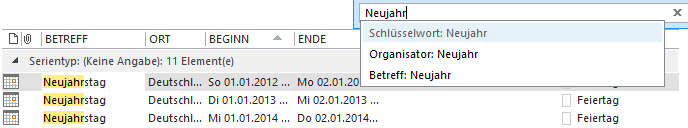
\includegraphics[width=\defaultFigureWidth]{outlook_search.png}
		\caption[Screenshot der Suche des Outlook"=Kalenders]{Screenshot der Suche des Outlook"=Kalenders von Microsoft Outlook 2013, Desktopversion}
		\label{fig:outlook_search}
	\end{margincap}
\end{figure}

Eine Funktion, welche beim Test der Suchfunktion auffällt, ist die automatische Aktualisierung der Trefferliste bei Veränderung des Suchbegriffs. Ohne die Suche aktiv starten zu müssen -- zum Beispiel über einen entsprechenden Button -- werden somit stets passende Veranstaltungen angezeigt. Dies könnte die notwendigen Tastaturanschläge bis zum gewünschten Suchergebnis minimieren.

Drückt man nach Eingabe eines Suchbegriffes die \keys{\arrowkeydown}-Taste, so wird ein Dropdownmenü angezeigt. Die Auswahl eines der unteren Einträge führt zu einer dynamischen Erweiterung des Suchbegriffes: \enquote{Organisator: Neujahr} ersetzt den Suchbegriff \texttt{Neujahr} durch \texttt{organisator:(Neujahr)}. Während standardmäßig alle Eigenschaften von Veranstaltungen durchsucht werden, kann die Suche hierdurch auf eine Spalte -- in diesem Beispiel den Organisator der Veranstaltung -- eingegrenzt werden. Zudem ist es ebenfalls möglich, selbst entsprechende Anfragen zu erstellen und durch Eingabe von \texttt{ort:(...)} die Suche auf den Veranstaltungsort zu beschränken. Das Menü stellt somit eine Möglichkeit dar, ohne Vorwissen komplexere Suchanfragen zu erzeugen.

Weitere Tests ergeben, dass die Suche auch boolesche Operatoren wie \texttt{AND} und \texttt{OR} unterstützt, die allerdings Case"=sensitiv sind. Während auf die Suchanfrage \texttt{betreff:(Neujahr) AND ort:(Land)} eine ähnliche Trefferliste wie in Abbildung \ref{fig:outlook_search} folgt, findet \texttt{betreff:(Neujahr) and ort:(Land)} keine einzige Veranstaltung.

Ebenfalls ins Auge sticht die Hervorhebung von Suchtreffern in der Auflistung der Veranstaltungen. Betrachtet man hierzu erneut den Screenshot \ref{fig:outlook_search}, so fällt die entsprechende gelbe Hinterlegung auf.

\subsubsection{Google}

Wenn auch keine direkte Veranstaltungssuche, so ist die Google Websuche doch eine verständliche Assoziation zum Begriff der Suchmaschine im Allgemeinen. Weshalb in diesem Abschnitt Bezug auf Google und nicht auf eine andere Suchmaschine genommen wird, veranschaulicht die Abbildung \ref{fig:websearchengines.market}.


\begin{figure}[ht!]
\begin{margincap}
	\centering
	\begin{tikzpicture}
	\begin{axis}[xbar, width=11cm, height=6cm, bar width=10pt,nodes near coords={\pgfmathprintnumber\pgfplotspointmeta\%}, nodes near coords align=horizontal, point meta=x * 1, legend pos=south east, xlabel=\textbf{Marktanteile von Websuchmaschinen},axis y line*=left,axis x line*=bottom, tick align=inside,  ytick={1,...,6},xmin=0,xmax=100,yticklabel style={/pgf/number format/fixed}, yticklabels={AOL Suche,Ask.com,T"=Online,Yahoo,Bing,Google}]
	\addplot[draw=ResponseOrange, fill=ResponseOrange] coordinates { (0.13,1) (0.18,2) (0.75,3) (1.66,4) (2.59,5) (94.84,6)};
	\end{axis}
	\end{tikzpicture}
	\caption[Marktanteile von Websuchmaschinen im Jahr 2015]{ Marktanteile von Websuchmaschinen im Jahr 2015 nach \cite[S. 31]{StatistaGmbH.September2014}}
	\label{fig:websearchengines.market}
\end{margincap}
\end{figure}

In Anbetracht des Marktanteils von über 90\,\% kommt Google eine gewisse Vormachtstellung zu. Dies sollte es legitimieren, konkurrierende Suchmaschinen für den Zweck dieses Abschnittes -- der Analyse von für den Benutzer gewohnten Referenzsystemen -- zu vernachlässigen.

Auffällig bei der Websuche über Google ist zum einen die Autovervollständigung: Nach Eingabe der Zeichenkette \enquote{Ingols} werden automatisch passende Vorschläge angezeigt, welche die Eingabe ergänzen -- in diesem Beispiel unter anderem zu \enquote{ingolstadt} und \enquote{ingolstadt today}.

\myMarginnote{Automatische Korrektur von Eingabefehlern}
Auch die automatische Rechtschreibkorrektur von Suchbegriffen zeigt eine mögliche Lösung der in Abschnitt \ref{sec:requirements_insite} beschriebenen Probleme. Ein fehlerhafter Suchbegriff wie \enquote{Inglstadt} führt zuerst zu einer Suche nach \enquote{ingolstadt}, Google weist auf den Fehler hin und bietet auch die Suche nach dem originalen -- fehlerhaften -- Suchbegriff an.


\subsection{Dokumente}
\label{sec:documents}

Auch vorliegende Dokumente können Basis für neue Anforderungen sein. \cite[S. 77]{Rupp.2014} nennt hierfür Normen oder Gesetzestexte. Lastenheft und Pflichtenheft listen ebenfalls Anforderungen an das zu erstellende Produkt auf \cite[S. 48f]{Grande.2014}.

Für ReEvent liegt derzeit kein Lasten- oder Pflichtenheft vor.\footnote{Stand 05.11.2015} Im Angebot\footnote{Stand 14.07.2009} wird spezifiziert: \enquote{Abbildung der bestehenden Funktionalität (INsite"=Veranstaltungen)}. INsite wiederum bietet sowohl im Backend als auch im Frontend lediglich eine einfache SQL"=basierte Suche an, welche um Filterkriterien ergänzt werden kann.\footnote{Vergleiche Abbildung \ref{fig:insite_screenshot_filter_original} aus dem Abschnitt \ref{sec:task}} Somit würde eine äquivalente SQL"=basierte Suche bereits den vertraglichen Anforderungen genügen.
%sind dem Landesdatenschutzgesetz unterworfen


%TODO
% \begin{itemize}
% 	\item Datenschutz - BayDSG / Cookies - Richtlinie 2009/136/EG
% 	\item Richtlinien des Rechenzentrums der Stadt Ingolstadt
% \end{itemize}
